\chapter{System Utilization of SDN/OpenFlow Controllers: Ryu Versus Pox}

    There are different SDN controllers available. Some of them are open source projects developed and maintained by the community, while private organizations develop some. Regardless of open source or private, all controllers follow the same principle of hardware independence and the divide and conquer approach. As with any case where there are multiple options of one thing, a choice is made because we cannot deploy all the options in the same environment simultaneously.
 
    To select the best controller, first, there is a need to understand the concept of the best controller. What are the criteria on which controllers need to be judged or compared? Is there even a possible best controller among them all. Similar to how we measure distance using a ruler, or time using a clock, we need a standard against which controllers can be compared, and then compare the comparisons with each other. This standard of metrics is crucial to selecting which controller would be ideal. There are some papers which mention a few relevant metrics, let us take a look.
    
    Controllers must be compared on several criteria. Previous papers discussed a wide variety of properties of controllers ranging from physical performance to fault tolerance. Some of the metrics include time for setting up the network, tearing down the network, processing power Usage, Potential to scale the network, CPU utilization, memory usage, throughput, latency, ping delay, no Response failure rate, a fair share of resources.
    
    These metrics give a fair idea of the performance of the controller on an industrial level. Nevertheless, all these criteria seem well researched and are continually evolving with upgraded hardware and new features in the software. Factors like system utilization also have to be evaluated to determine whether the controller uses the hardware constraints efficiently. It also gives a clear idea about the controller's nature while it is running and helps identify the system bottlenecks.
    
    A paper published in 2018 came up with methodologies for measuring the performance of all controller implementations and benchmarked the control- plane performance \cite{rfc8456}.
    
    Another paper, published in 2019, describes a repetitive series of tests using a network emulator and a benchmark tool that included the CPU utilization of various Controllers on a machine. It uses a benchmark tool which operates on a different system, that sends a considerable amount of random packets to the controller and then reads CPU utilization values. Fig. \ref{figzhu2019sdn} below depicts the average CPU utilization at a given time. The graph gets populated by data from the benchmark tool, which performs the test seamlessly. At the same time, the controller operating system runs on a virtual machine \cite{zhu2019sdn}. Currently, the benchmark OFNet used in that experiment is no longer available as the concerned owner has removed it.
    
    A paper, published in 2014, describes how OFCBench and OFCProbe can be used as CPU and RAM utilization monitor and find bottlenecks of the controller. The implementation of these monitors is by sending SMTP messages from client machines. However, it is worth noting that both these tools are limited to work with Floodlight, Ryu, and Nox Controllers. \cite{ofcprobe}
    
    One more paper, published in 2012, shows they used multiple instances of CBench to send packets and measure the CPU Utilization. They discovered an inherent performance bottleneck concerning CPU load in OpenFlow switch implementations of those days. \cite{flexible}
    
\begin{figure}[!hbt]
    \centering
        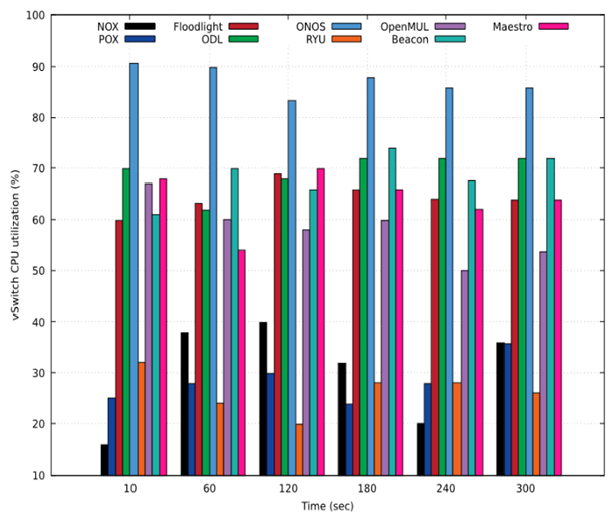
\includegraphics[width=\textwidth,keepaspectratio]{images/zhucpu.png}
       \caption{CPU Utilization Results Published \cite{zhu2019sdn}}
        \label{figzhu2019sdn}
\end{figure}

    The throughput mode of CBench in which the switches are configured to wait and pile up a set of requests and send all the requests at once to the controller. This forces the controller to allocate a significant share of its resources to one or two switches at a time. This technique measures the stress capacity of the controller. The controller must have enough memory to store and process all the requests from a switch. It need not be able to run so many threads at the same time.

    The tests performed in the paper \cite{dynamicrouting} consider many controllers, running in a network whose size increases. For this feature, they increased the number of nodes after each set of tests and repeated them while recording the results. The thing that seems overlooked in this test is that the results are valid, provide us only with a basic idea of the controller's performance. The controller with the best growth of response rate in proportion to network size was classified as the best controller.
        
    The controller provides more responses as the network size increase. It is because there is more packet in events from switches. As the network size increases, more routes need to be calculated and maintained. More switches need to be updated regularly. However, one factor is overlooked. The fact that more requests are generated is not necessarily because there are more switches; it is because there are more hosts overall connected to the network. The experiment performed as in paper \cite{routingtie2017} by increasing the number of switches while maintaining the number of hosts per switch. As the network grew, more hosts would want to communicate, thus leading to the rise in route requests or packet in events.
    
    \textit{Traffic Intensity} is a measure of how flooded a network is with traffic. As the network gets scaled up, the number of hosts increases, thus increasing traffic Intensity. This increase in traffic intensity forces the controller to increase its performance rates to cope with the network requirements. There is a need for a method to compare controller such that minimum external factors are influencing the controller's performance. Here, the traffic Intensity is kept quite high, changing the network topology to see how different controllers handle the scenario and how their performance is affected.

    For any test, the environment within which the subject to be tested must be isolated from external factors as much as possible. In the case of testing and performing a benchmark on SDN controllers, the cores of CPU where the controller runs, needs to be isolated using \textit{isolcpus} or similar tool.